\documentclass[11pt]{article}
\usepackage{fullpage}
\usepackage{amsfonts}
\usepackage{amsmath}
\usepackage{amsthm}
\usepackage{graphicx}
\usepackage{ulem}
\usepackage{framed}
\usepackage{url}

% Command for independent symbol
\def\ci{\perp}

% Command for not independent symbol
\def\notci{\not\perp}

% Packages for graphs and arrows
\usepackage{tikz}
\usetikzlibrary{arrows, calc, positioning, fit}

% Package for forcing figure placement
\usepackage{float}

\begin{document}

\title{CS 5526 -- Virginia Tech\\
	Homework 2}
\author{Brennon Bortz \\ (PID: brennon, Campus: Blacksburg)}
\date{1 April 2015}
\maketitle

Code for this assignment is available at \url{https://github.com/brennon/cs5526-hw2}.

\section*{Written Problems}

\begin{enumerate}

\item (10 points) Prove that the dimensionality of the feature space for the inhomogeneous polynomial kernel of degree $q$ is

\begin{equation}
m = \binom{d+q}{q} \nonumber
\end{equation}

\textbf{Solution:} Per the text, the mapping $\phi : \mathbb{R}^d \rightarrow \mathbb{R}^m$ is given as the vector

\begin{equation}
\phi(\mathbf{x}) = (\ldots , a_n \mathbf{x}^\mathbf{n} , \ldots)^\mathit{T} = \cdots \nonumber
\end{equation}

where the variable $\mathbf{n}=(n_0,\ldots,n_d)$ ranges over all the possible assignments such that $|\mathbf{n}|=q$ (the sum of $\mathbf{n}$ equals $q$). This is equivalent to the number of monomial terms in a multinomial expansion, and can be counted by the stars and bars method.

To illustrate this, let $q = 5$ and $d = 3$. We are searching for all assignments of non-negative integers to the values $n_0,\ldots,n_d$ such that they sum to $q$. Arrange 5 stars (*) in a row. Place 4 bars (as there are $d + 1$ terms in $n_0,\ldots,n_d$) (|) between any of the stars, to the left of the entire row of stars, or to the right of the entire row of stars. Moving from left to right, groups of stars are counted and assigned to each $n_i$. Where there are no stars between two bars, the value of 0 is given to the corresponding $n_i$.

There are $\binom{d+1+q-1}{q} = \binom{d+q}{q}$ ways to arrange the stars and bars, and thus there are $\binom{d+q}{q}$ assignments of non-negative integers to the values $n_0,\ldots,n_d$ such that they sum to $q$.

\item (12 points) Given the three points $\mathbf{x}_1 = (2.5, 1)^\mathit{T}$, $\mathbf{x}_1 = (3.5, 4)^\mathit{T}$, and $\mathbf{x}_1 = (2, 2.1)^\mathit{T}$.

\begin{enumerate}
\item Compute the kernel matrix for the Gaussian kernel assuming that $\sigma^2 = 5$.

\begin{eqnarray*}
K(\mathbf{x}_1, \mathbf{x}_1) &=& \text{exp} \left( \frac{\left \Vert \left( \begin{array}{cc} 2.5 & 1 \end{array} \right) - \left( \begin{array}{cc} 2.5 & 1 \end{array} \right) \right \Vert^2}{10} \right) \\ \nonumber
&=& \text{exp} \left( \frac{\left \Vert \left( \begin{array}{cc} 0 & 0 \end{array} \right) \right \Vert^2}{10} \right) \\ \nonumber
&=& \text{exp} \left( - \frac{0}{10} \right) \\ \nonumber
&=& \text{exp} \left( 0 \right) \\
&=& 1 \nonumber
\end{eqnarray*}

Similar computations show that $K(\mathbf{x}_1, \mathbf{x}_1) = K(\mathbf{x}_2, \mathbf{x}_2) = K(\mathbf{x}_3, \mathbf{x}_3) = 1$.

\begin{eqnarray*}
K(\mathbf{x}_2, \mathbf{x}_1) = K(\mathbf{x}_1, \mathbf{x}_2) &=& \text{exp} \left( \frac{\left \Vert \left( \begin{array}{cc} 2.5 & 1 \end{array} \right) - \left( \begin{array}{cc} 3.5 & 4 \end{array} \right) \right \Vert^2}{10} \right) \\ \nonumber
&=& \text{exp} \left( \frac{\left \Vert \left( \begin{array}{cc} -1 & -3 \end{array} \right) \right \Vert^2}{10} \right) \\ \nonumber
&=& \text{exp} \left( - \frac{\sqrt{10}^2}{10} \right) \\ \nonumber
&=& \text{exp} \left( -1 \right) \\ \nonumber
&=& 0.3679
\end{eqnarray*}

\begin{eqnarray*}
K(\mathbf{x}_3, \mathbf{x}_1) = K(\mathbf{x}_1, \mathbf{x}_3) &=& \text{exp} \left( \frac{\left \Vert \left( \begin{array}{cc} 2.5 & 1 \end{array} \right) - \left( \begin{array}{cc} 2.5 & 2.1 \end{array} \right) \right \Vert^2}{10} \right) \\ \nonumber
&=& \text{exp} \left( \frac{\left \Vert \left( \begin{array}{cc} 0.5 & -1.1 \end{array} \right) \right \Vert^2}{10} \right) \\ \nonumber
&=& \text{exp} \left( - \frac{\sqrt{1.46}^2}{10} \right) \\ \nonumber
&=& \text{exp} \left( -0.146 \right) \\ \nonumber
&=& 0.8642
\end{eqnarray*}

\begin{eqnarray*}
K(\mathbf{x}_3, \mathbf{x}_2) = K(\mathbf{x}_2, \mathbf{x}_3) &=& \text{exp} \left( \frac{\left \Vert \left( \begin{array}{cc} 3.5 & 4 \end{array} \right) - \left( \begin{array}{cc} 2 & 2.1 \end{array} \right) \right \Vert^2}{10} \right) \\ \nonumber
&=& \text{exp} \left( \frac{\left \Vert \left( \begin{array}{cc} 1.5 & 1.9 \end{array} \right) \right \Vert^2}{10} \right) \\ \nonumber
&=& \text{exp} \left( - \frac{\sqrt{5.86}^2}{10} \right) \\ \nonumber
&=& \text{exp} \left( -0.586 \right) \\ \nonumber
&=& 0.5565
\end{eqnarray*}

Putting these together, we have

\begin{equation*}
K = \left[ \begin{array}{ccc}
1 & 0.3679 & 0.8642 \\
0.3679 & 1 & 0.5565 \\
0.8642 & 0.5565 & 1 \\
\end{array} \right]
\end{equation*}

\textbf{Solution:}

\item Compute the distance of the point $\phi(\mathbf{x}_1)$ from the mean in feature space.

\textbf{Solution:}

\begin{equation*}
\Vert \phi(\mathbf{x}_1) - \mu_\phi \Vert^2 = K(\mathbf{x}_1,\mathbf{x}_1) - \frac{2}{n} \sum\limits_{j=1}^n K(\mathbf{x}_1,\mathbf{x}_j) + \frac{1}{n^2} \sum\limits_{a=1}^n \sum\limits_{b=1}^n K(\mathbf{x}_a,\mathbf{x}_b)
\end{equation*}

\begin{eqnarray*}
\frac{1}{n^2} \sum\limits_{a=1}^n \sum\limits_{b=1}^n K(\mathbf{x}_a,\mathbf{x}_b) 
&=& \frac{1}{3^2} \left[ 1 + 0.3679 + 0.8642 + 0.3679 + 1 + 0.5565 + 0.8642 + 0.5565 + 1 \right] \\
&=& \frac{6.5572}{9} \\
&=& 0.7308
\end{eqnarray*}

\begin{eqnarray*}
\frac{2}{n} \sum\limits_{j=1}^n K(\mathbf{x}_1,\mathbf{x}_j) &=& \frac{2}{3} \left[1 + 0.3679 + 0.8642 \right] \\
&=& \frac{2.2321}{3} = 1.4881 \\
\end{eqnarray*}

\begin{eqnarray*}
\Vert \phi(\mathbf{x}_1) - \mu_\phi \Vert^2 &=& 1.0 - 1.4881 + 0.7308 \\
&=& 0.2427 \\
\Vert \phi(\mathbf{x}_1) - \mu_\phi \Vert &=& 0.2427^2 = 0.0589
\end{eqnarray*}

\item Compute the dominant eigenvector and eigenvalue for the kernel matrix from (a).

\textbf{Solution:}

MATLAB gives the following eigenvalues for the matrix in (a): 0.1084, 0.674, and 2.2176. The corresponding eigenvector for the domninant eigenvalue (2.2176) is:

\begin{equation*}
\left(\begin{array}{c}
0.6002 \\
0.4754 \\
0.6433 \\
\end{array}\right)
\end{equation*}

\end{enumerate}

\item (30 points) Consider the dataset in Figure 21.9 (shown in the text), which has points from two classes $c_1$ (triangles) and $c_2$ (circles). Answer the questions below.

\begin{enumerate}
\item Find the equations for the two hyperplanes $h_1$ and $h_2$.

\textbf{Solution:}

We use the points $x_1 = (\begin{array}{cc}6 & 0 \end{array})$ and $x_2 = (\begin{array}{cc}5 & 2 \end{array})$ on $h_1$ to find the equation for $h_1$

\begin{equation*}
h_1 = \mathbf{w}^\mathit{T} \mathbf{x} + b = w_1 x_1 + w_2 x_2 + b = 0
\end{equation*}

Rearranging terms

\begin{equation*}
x_2 = - \frac{w_1}{w_2} x_1 - \frac{b}{w_2}
\end{equation*}

where $- \frac{w_1}{w_2}$ is the slope of the line, and $- \frac{b}{w_2}$ is the intercept along the second dimension.

\begin{equation*}
-\frac{w_1}{w_2} = \frac{2-0}{5-6} = -\frac{2}{1}
\end{equation*}

which implies that $w_1 = 2$ and $w_2 = 1$. We compute the offset $b$ directly

\begin{equation*}
b = - 2 x_1 - 1 x_2 = -2 \cdot 6 - 1 \cdot 0 = -12
\end{equation*}

Thus, $\mathbf{w} = \left( \begin{array}{c} 2 \\ 1 \end{array} \right)$ is the weight vector, and $b = -12$ is the bias, and the equation of the hyperplane is given as

\begin{equation*}
h(\mathbf{x}) = \mathbf{w}^\mathit{T} \mathbf{x} + b = (\begin{array}{cc} 2 & 1 \end{array}) \left( \begin{array}{c} x_1 \\ x_2 \end{array} \right) - 12 = 0
\end{equation*}

We use the points $x_1 = (\begin{array}{cc}2 & 0 \end{array})$ and $x_2 = (\begin{array}{cc}5 & 5 \end{array})$ on $h_1$ to find the equation for $h_1$

\begin{equation*}
-\frac{w_1}{w_2} = \frac{5-0}{5-2} = \frac{5}{3}
\end{equation*}

which implies that $w_1 = -5$ and $w_2 = 3$. We compute the offset $b$ directly

\begin{equation*}
b = - (-5) x_1 - 3 x_2 = 5 \cdot 5 - 3 \cdot 5 = 10
\end{equation*}

Thus, $\mathbf{w} = \left( \begin{array}{c} -5 \\ 3 \end{array} \right)$ is the weight vector, and $b = 10$ is the bias, and the equation of the hyperplane is given as

\begin{equation*}
h(\mathbf{x}) = \mathbf{w}^\mathit{T} \mathbf{x} + b = (\begin{array}{cc} -5 & 3 \end{array}) \left( \begin{array}{c} x_1 \\ x_2 \end{array} \right) + 10 = 0
\end{equation*}

\item Show all the support vectors for $h_1$ and $h_2$.

\textbf{Solution:}

The support vectors for $h_1$ are $(\begin{array}{cc} 2 & 6 \end{array})$, $(\begin{array}{cc} 3 & 4 \end{array})$, and $(\begin{array}{cc} 6 & 2 \end{array})$.

The support vectors for $h_2$ are $(\begin{array}{cc} 3 & 4 \end{array})$ and $(\begin{array}{cc} 7 & 6 \end{array})$.

\item Which of the two hyperplanes is better at separating the two classes based on the margin computation?

To find the margin of each hyperplane, we must first find the canonical hyperplanes for $h_1$ and $h_2$.

The equation of the separating hyperplane $h_1$ is

\begin{equation*}
h_1(\mathbf{x}) = \left( \begin{array}{c} 2 \\ 1 \end{array} \right) \mathbf{x} - 12 = 0
\end{equation*}

Consider the support vector $\mathbf{x}^* = (3,4)^\mathit{T}$, with class $y^* = -1$. To find the canonical hyperplane equation, we have to rescale the weight vector and bias by the scalar $s$

\begin{equation*}
s = \frac{1}{y^*h_1(\mathbf{x}^*)} = \frac{1}{-1\left(
\left(
\begin{array}{c}
2 \\ 1
\end{array}
\right)^\mathit{T}
\left(
\begin{array}{c}
3 \\ 4
\end{array}
\right) - 12 \right)}
=
\frac{1}{2}
\end{equation*}

Thus, the rescaled weight vector is

\begin{equation*}
\mathbf{w} = \frac{1}{2}
\left(
\begin{array}{c}
2 \\ 1
\end{array}
\right)
=
\left(
\begin{array}{c}
1 \\ 1
\end{array}
\right)
\end{equation*}

and the rescaled bias is

\begin{equation*}
b = \frac{1}{2} \cdot -12 = -6
\end{equation*}

The canonical form of the hyperplane is therefore

\begin{equation*}
h_1(\mathbf{x}) = \mathbf{x} - 6
\end{equation*}

and the margin of the canonical hyperplane for $h_1$ is

\begin{equation*}
\delta^*
=
\frac{y^*h(\mathbf{x}^*)}{\Vert \mathbf{w} \Vert}
=
\frac{1}{1}
=
1
\end{equation*}

The equation of the separating hyperplane $h_2$ is

\begin{equation*}
h_2(\mathbf{x}) = \left( \begin{array}{c} -5 \\ 3 \end{array} \right) \mathbf{x} + 10 = 0
\end{equation*}

Consider the support vector $\mathbf{x}^* = (3,4)^\mathit{T}$, with class $y^* = -1$. To find the canonical hyperplane equation, we have to rescale the weight vector and bias by the scalar $s$

\begin{equation*}
s = \frac{1}{y^*h_2(\mathbf{x}^*)} = \frac{1}{-1\left(
\left(
\begin{array}{c}
-5 \\ 3
\end{array}
\right)^\mathit{T}
\left(
\begin{array}{c}
3 \\ 4
\end{array}
\right) + 10 \right)}
=
\frac{1}{-1 (-3 + 10)}
=
-\frac{1}{7}
\end{equation*}

Thus, the rescaled weight vector is

\begin{equation*}
\mathbf{w} = -\frac{1}{7}
\left(
\begin{array}{c}
-5 \\ 3
\end{array}
\right)
=
\left(
\begin{array}{c}
5/7 \\ -3/7
\end{array}
\right)
\end{equation*}

and the rescaled bias is

\begin{equation*}
b = -\frac{1}{7} \cdot 10 = -\frac{10}{7}
\end{equation*}

The canonical form of the hyperplane is therefore

\begin{equation*}
h_2(\mathbf{x})
=
\left(\begin{array}{c}
5/7 \\ -3/7
\end{array}\right)^\mathit{T} \mathbf{x} - \frac{10}{7}
=
\left(\begin{array}{c}
0.7143 \\ -0.4286
\end{array}\right)^\mathit{T} \mathbf{x} - 1.4286
\end{equation*}

and the margin of the canonical hyperplane for $h_2$ is

\begin{equation*}
\delta^*
=
\frac{y^*h(\mathbf{x}^*)}{\Vert \mathbf{w} \Vert}
=
\frac{1}{\sqrt{0.7143^2 + (-0.4286)^2}}
=
\frac{1}{\sqrt{0.5102 + 0.1387}}
=
\frac{1}{0.6489}
=
-1.5411
\end{equation*}

Thus, the hyperplane $h_2$ is better at separating the two classes based on these margin computations.

\textbf{Solution:}

\item Find the equation of the best separating hyperplane for this dataset, and show the corresponding support vectors. You can do this without having to solve the Lagrangian by considering the convex hull of each class and the possible hyperplanes at the boundary of the two classes.

\textbf{Solution:}

Based on the latter approach suggested in the problem, two of the points on the best separating hyperplane are $x_1 = (4.5, 2)$ and $x_2 = (5.5, 6)$. Following the logic from part (a) we use these points to find the equation for this new separating hyperplane $h_3$

\begin{equation*}
h_3 = \mathbf{w}^\mathit{T} \mathbf{x} + b = w_1 x_1 + w_2 x_2 + b = 0
\end{equation*}

Rearranging terms

\begin{equation*}
x_2 = - \frac{w_1}{w_2} x_1 - \frac{b}{w_2}
\end{equation*}

where $- \frac{w_1}{w_2}$ is the slope of the line, and $- \frac{b}{w_2}$ is the intercept along the second dimension.

\begin{equation*}
-\frac{w_1}{w_2} = \frac{6-2}{5.5-4.5} = \frac{4}{1}
\end{equation*}

which implies that $w_1 = -4$ and $w_2 = 1$. We compute the offset $b$ directly

\begin{equation*}
b = 4 x_1 - 1 x_2 = 4 \cdot 4.5 - 1 \cdot 2 = 18 - 2 = 16
\end{equation*}

Thus, $\mathbf{w} = \left( \begin{array}{c} -4 \\ 1 \end{array} \right)$ is the weight vector, and $b = 16$ is the bias, and the equation of the hyperplane is given as

\begin{equation*}
h(\mathbf{x}) = \mathbf{w}^\mathit{T} \mathbf{x} + b = (\begin{array}{cc} -4 & 1 \end{array}) \left( \begin{array}{c} x_1 \\ x_2 \end{array} \right) + 16 = 0
\end{equation*}

\end{enumerate}

\item (18 points) Given the 10 points in Table 21.2 (shown in the text), along with their classes and their Lagranian multipliers ($\alpha_i$), answer the following questions:

\begin{enumerate}
\item What is the equation of the SVM hyperplane $h(x)$?

\textbf{Solution:}

We compute the weight vector for the hyperplane with

\begin{eqnarray*}
\mathbf{w} &=& \sum\limits_{i,\alpha_i > 0} \alpha_i y_i \mathbf{x}_i \\
&=& 0.414 \left( \begin{array}{c} 4 \\ 2.9 \end{array} \right) 
-0.018 \left( \begin{array}{c} 2.5 \\ 1 \end{array} \right)
+0.018 \left( \begin{array}{c} 3.5 \\ 4 \end{array} \right)
-0.414 \left( \begin{array}{c} 2 \\ 2.1 \end{array} \right) \\
&=& \left( \begin{array}{c} 0.846 \\ 0.3852 \end{array} \right)
\end{eqnarray*}

The final bias is the average of the bias obtained from each support vector using

\begin{equation*}
b_i = y_i - \mathbf{w}^\mathit{T} \mathbf{x}_i
\end{equation*}

\begin{eqnarray*}
b_1 &=& 
1 - \left( \begin{array}{c} 0.846 \\ 0.3852 \end{array} \right)^\mathit{T}
\left( \begin{array}{c} 4 \\ 2.9 \end{array} \right)
= -1.22692 \\
b_4 &=& 
-1 - \left( \begin{array}{c} 0.846 \\ 0.3852 \end{array} \right)^\mathit{T}
\left( \begin{array}{c} 2.5 \\ 1 \end{array} \right)
= -2.7298 \\
b_7 &=& 
1 - \left( \begin{array}{c} 0.846 \\ 0.3852 \end{array} \right)^\mathit{T}
\left( \begin{array}{c} 3.5 \\ 4 \end{array} \right)
= -0.4202 \\
b_9 &=& 
-1 - \left( \begin{array}{c} 0.846 \\ 0.3852 \end{array} \right)^\mathit{T}
\left( \begin{array}{c} 2 \\ 2.1 \end{array} \right)
= -1.88308 \\
b &=& \text{avg}(b_i) = -1.575
\end{eqnarray*}

Thus, the optimal hyperplane is given as follows:

\begin{equation*}
h(\mathbf{x}) = \left( \begin{array}{c} 0.846 \\ 0.3852 \end{array} \right)^\mathit{T} \mathbf{x} - 1.575 = 0
\end{equation*}

\item What is the distance of $x_6$ from the hyperplane? Is it within the margin of the classifier?

\textbf{Solution:}

To compute this distance \textit{and} determine whether or not it lies in the margin, we must first find the canonical form of the separating hyperplane. The equation of the separating hyperplane $h$ is

\begin{equation*}
h(\mathbf{x}) = \left( \begin{array}{c} 0.846 \\ 0.3852 \end{array} \right)^\mathit{T} \mathbf{x} - 1.575 = 0
\end{equation*}

Consider the support vector $\mathbf{x}^* = \mathbf{x}_1 = (4,2.9)^\mathit{T}$, with class $y^* = 1$. To find the canonical hyperplane equation, we have to rescale the weight vector and bias by the scalar $s$

\begin{equation*}
s = \frac{1}{y^*h_1(\mathbf{x}^*)} = \frac{1}{1\left(
\left(
\begin{array}{c}
0.846 \\ 0.3852
\end{array}
\right)^\mathit{T}
\left(
\begin{array}{c}
4 \\ 2.9
\end{array}
\right) - 1.575 \right)}
=
\frac{1}{4.5018 - 1.575}
=
\frac{1}{2.92608}
=
0.3418
\end{equation*}

Thus, the rescaled weight vector is

\begin{equation*}
\mathbf{w} = 0.3418
\left(
\begin{array}{c}
0.846 \\ 0.3852
\end{array}
\right)
=
\left(
\begin{array}{c}
0.2892 \\ 0.1317
\end{array}
\right)
\end{equation*}

and the rescaled bias is

\begin{equation*}
b = 0.348 \cdot -1.575 = -0.5383
\end{equation*}

The canonical form of the hyperplane is therefore

\begin{equation*}
h(\mathbf{x}) = 
\left(
\begin{array}{c}
0.2892 \\ 0.1317
\end{array}^\mathit{T}
\right)
\mathbf{x} - 0.5383
\end{equation*}

and the margin of the canonical hyperplane for $h$ is

\begin{equation*}
\delta^*
=
\frac{y^*h(\mathbf{x}^*)}{\Vert \mathbf{w} \Vert}
=
\frac{1}{\sqrt{0.2892^2 + 0.1317^2}}
=
\frac{1}{\sqrt{0.0836 + 0.0173}}
=
\frac{1}{\sqrt{0.1009}}
=
0.3176
\end{equation*}

The distance from $\mathbf{x}_6$ to the hyperplane is then given by

\begin{eqnarray*}
\delta^*
&=&
\frac{y_6(\mathbf{x}_6)}{\Vert \mathbf{w} \Vert}
=
\frac{
-1
\left(
\begin{array}{c}
0.2892 \\ 0.1317
\end{array}^\mathit{T}
\right)
\left(
\begin{array}{c}
1.9 \\ 1.9
\end{array}
\right) - 0.5383
}{0.3176} \\
&=& \frac{-1 \cdot 0.79971 - 0.5383}{0.3176} \\
&=& \frac{-1.33801}{0.3176} \\
&=& -4.2129
\end{eqnarray*}

While the SVM misclassifies $\mathbf{x}_6$, it does not lie within the SVM margin.

\item Classify the point $\mathbf{z} = (3, 3)_\mathit{T}$ using $h(x)$ from above.

\textbf{Solution:}

We classify the point $\mathbf{z}$ by

\begin{eqnarray*}
\hat{y} &=& \text{sign}(h(\mathbf{z})) \\
&=& \text{sign}( \mathbf{w}^\mathit{T} \mathbf{z} + b ) \\
&=& \text{sign}\left( \left( \begin{array}{c} 0.2892 \\ 0.1317 \end{array} \right)^\mathit{T} \left( \begin{array}{c} 3 \\ 3 \end{array} \right) - 0.5383 \right) \\
&=& \text{sign}(1.2627 - 0.5383) \\
&=& \text{sign}(0.7244) \\
&=& +
\end{eqnarray*}

\end{enumerate}

\item (30 points) Create a binary (2 feature) dataset where the target (2-class) variable encodes the XOR function. Design and implement a SVM (with a suitable kernel) to learn a classifier for this dataset. For full credit, explain the kernel you selected, and the support vectors picked by the algorithm. Redo all the above with multiple settings involving more than 2 features. Ensure that your kernel is able to model XOR in all these dimensions. Now begin deleting the non-support vectors from your dataset and relearn the classifier. What do you observe? Does the margin increase or decrease? What will happen to the margin if the support vectors are removed from the dataset? Will the margin increase or decrease?

\textbf{Solution:} Code for this question is provided at the URL listed at the beginning of this document.

I selected a Gaussian kernel for use with SVM, and trained the classifier using the dual SVM stochastic gradient descent algorithm provided by Zaki and Meira. In addition, the SVM was trained with $C = 10$ and $\epsilon = .00001$. The SVM was trained and tested on datasets with input feature dimensions ranging from 2 to 32. Figure \ref{fig:features_vs_accuracy} shows accuracies obtained using hold-out cross-validation on datasets across this range of input feature dimensions. All datasets included 500 examples, with 67\% of examples used for training and 33\% used for testing.

\begin{figure}[H]
    \centering
    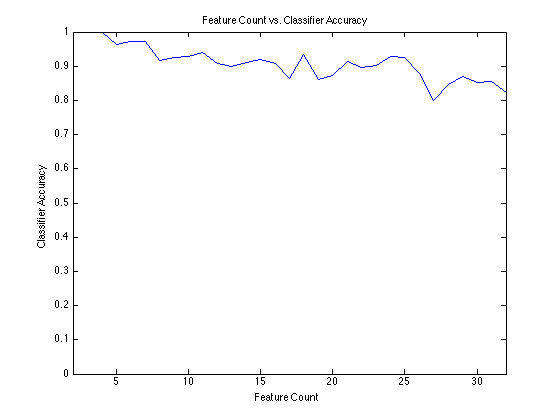
\includegraphics[width=0.5\textwidth]{features_vs_accuracy.png}
    \caption{Input dimensionality vs. accuracy.}
    \label{fig:features_vs_accuracy}
\end{figure}

Overall, the classifier performs very well, with a mean accuracy of 91\% across all dimensionalities. At the higher end of the range of input dimensionality, accuracy begins to drop, but never below 80\%. With an input feature dimensionality of 32, a dataset with 500 examples can only represent .0001\% of possible examples, in the best case scenario. Thus, even at this extreme end of the range, an accuracy of $> 80\%$ is very respectable.

The support vectors selected by the classifier are mostly the positive examples (those that pass the XOR test) on one side of the separating hyperplane, and the zero vector and points with a `smaller' number of ones. Figure \ref{fig:support_vectors} characterizes the selected support vectors for a classifier where the input space is in $\mathbb{R}^8$. Here, most of the support vectors are those points with one one, and on the other side of the hyperplane we have support vectors with 0, 2, 3, and 4 ones. No points with $>4$ ones are selected as support vectors.

\begin{figure}[H]
    \centering
    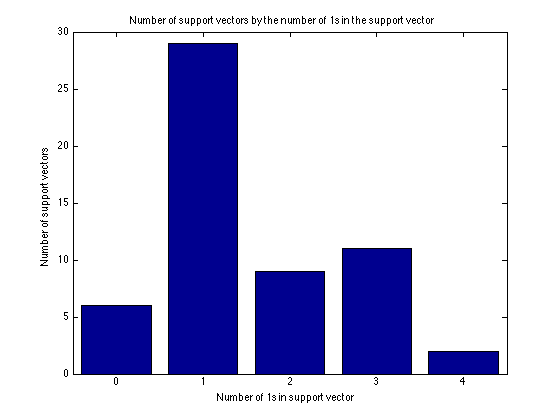
\includegraphics[width=0.5\textwidth]{support_vectors.png}
    \caption{Support vector characteristics.}
    \label{fig:support_vectors}
\end{figure}

Removing both points that are support vectors and points that are not support vectors does little to affect the accuracy of the classifier, as Figures \ref{fig:removed_nsvs} and \ref{fig:removed_svs} demonstrate, respectively. As I have selected a kernel that produces an infinite feature space, it is impossible to reconstruct $\mathbf{w}$ in the input space, and thus impossible to determine the margin, per Zaki and Meira. In fact, it is even difficult to characterize the concept of a margin in infinite feature space.

My intuition tells me the following, however. As points that are not support vectors are removed from the dataset, the original support vectors still remain, and thus the margin should remain unchanged. On the other hand, as points that \textit{are} support vectors are removed from the dataset, the SVM has a wider `gap' across which to reach in order to find support vectors, and thus the margin should widen, in turn. Figure \ref{fig:removed_svs} reinforces this intuition, as when most support vectors are removed from the dataset, the accuracy of the classifier trends toward 100\%.

\begin{figure}[H]
    \centering
    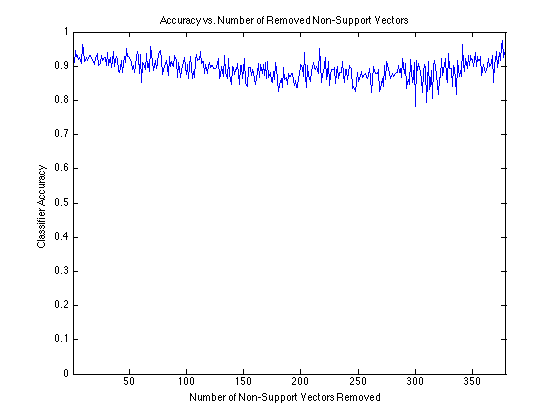
\includegraphics[width=0.5\textwidth]{removed_nsvs.png}
    \caption{Effect of removing points that \textit{are not} support vectors from the dataset.}
    \label{fig:removed_nsvs}
\end{figure}

\begin{figure}[H]
    \centering
    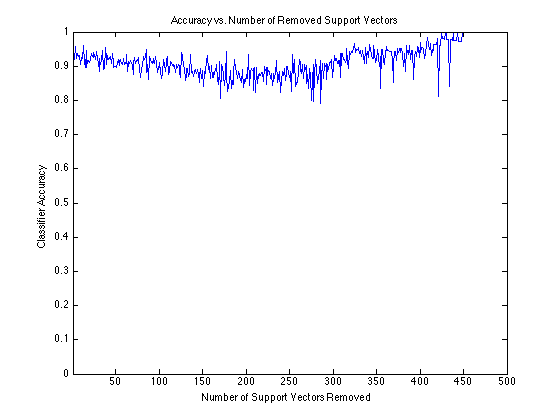
\includegraphics[width=0.5\textwidth]{removed_svs.png}
    \caption{Effect of removing points that \textit{are} support vectors from the dataset.}
    \label{fig:removed_svs}
\end{figure}

%\textbf{Solution:} The graph structure of Figure \ref{fig:impossible} with the following as the only independencies cannot be represented by a Bayesian network: $(A \ci D | B,C)$ and $(B \ci C | A,D)$.
%
%\begin{figure}[H]
%\centering
%\begin{tikzpicture}[-,>=stealth',shorten >=1pt,auto,node distance=3cm,
%                    thick,main node/.style={circle,draw,font=\sffamily\Large\bfseries}]
%
%  \node[main node] (A) {$A$};
%  \node[main node] (B) [below left of=A] {$B$};
%  \node[main node] (C) [below right of=A] {$C$};
%  \node[main node] (D) [below right of=B] {$D$};
%
%  \path[every node/.style={font=\sffamily\small}]
%    (A) edge node [] {} (B)
%    (A) edge node [] {} (C)
%    (C) edge node [] {} (D)
%    (B) edge node [] {} (D);
%    
%\end{tikzpicture}
%\caption{Impossible Bayesian network.}
%\label{fig:impossible}
%\end{figure}
%
%\item (10 points) How many possible Bayesian networks are there involving three random variables? Group these networks into equivalence classes where each class contains networks that encode the same (conditional) independence assumptions.
%
%\textbf{Solution:} There are 25 possible Bayesian networks involving three variables, comprising 8 different equivalence classes. Each row in Table \ref{fig:possible} shows one of these possible networks. An arrow in one of the first three columns indicates the direction of the edge connecting the nodes given in the header row. A check in one of the last three columns indicates the conditional independency in the header row holds given the edges indicated in the first three columns. Where two rows share the same pattern of check in the last three columns, they are members of the same equivalence class.
%
%\begin{table}[h]
%\centering
%\begin{tabular}{c|c|c||c|c|c}
%X-Y & Y-Z  & X-Z & $X \ci Y | Z$ & $X \ci Z | Y$ & $Y \ci Z | X$ \\
%\hline
% &  &  & $\checkmark$ & $\checkmark$ & $\checkmark$\\
% & $\leftarrow$ &  & $\checkmark$ & $\checkmark$ & \\
% & $\rightarrow$ &  & $\checkmark$ & $\checkmark$ & \\
% &  & $\leftarrow$ & $\checkmark$ &  & $\checkmark$\\
% &  & $\rightarrow$ & $\checkmark$ &  & $\checkmark$\\
% & $\leftarrow$ & $\rightarrow$ & $\checkmark$ &  & \\
% & $\rightarrow$ & $\leftarrow$ & $\checkmark$ &  & \\
%$\leftarrow$ &  &  &  & $\checkmark$ & $\checkmark$\\
%$\rightarrow$ &  &  &  & $\checkmark$ & $\checkmark$\\
% & $\leftarrow$ & $\leftarrow$ &  & $\checkmark$ & \\
%$\leftarrow$ & $\leftarrow$ &  &  & $\checkmark$ & \\
%$\leftarrow$ & $\rightarrow$ &  &  & $\checkmark$ & \\
%$\rightarrow$ & $\rightarrow$ &  &  & $\checkmark$ & \\
%$\leftarrow$ &  & $\rightarrow$ &  &  & $\checkmark$\\
%$\rightarrow$ &  & $\leftarrow$ &  &  & $\checkmark$\\
%$\rightarrow$ &  & $\rightarrow$ &  &  & $\checkmark$\\
% & $\rightarrow$ & $\rightarrow$ &  &  & \\
%$\leftarrow$ &  & $\leftarrow$ &  &  & \\
%$\leftarrow$ & $\leftarrow$ & $\leftarrow$ &  &  & \\
%$\leftarrow$ & $\rightarrow$ & $\leftarrow$ &  &  & \\
%$\leftarrow$ & $\rightarrow$ & $\rightarrow$ &  &  & \\
%$\rightarrow$ & $\leftarrow$ &  &  &  & \\
%$\rightarrow$ & $\leftarrow$ & $\leftarrow$ &  &  & \\
%$\rightarrow$ & $\leftarrow$ & $\rightarrow$ &  &  & \\
%$\rightarrow$ & $\rightarrow$ & $\rightarrow$ &  &  & 
%\end{tabular}
%\caption{Possible Bayesian networks in three variables.}
%\label{fig:possible}
%\end{table}
%
%\item (10 points) In the attached diagram (next page) assume that B and M are instantiated (i.e., evidence is introduced for these variables). List all the random variables that A is conditionally independent of.
%
%\textbf{Solution:} $A$ is only independent of $G$ given $B$ and $M$.
%
%\item (20 points) From Project Gutenberg, download the two files The Adventures of Sherlock Holmes by Arthur Conan Doyle (http://www.gutenberg.org/cache/epub/1661/pg1661.txt) and The Complete Works of Jane Austen (http://www.gutenberg.org/cache/epub/31100/pg31100.txt). Design a Markov sequence model that learns from each of these files (separately) and learns to write like Doyle or write like Austen. Note that your model need not be a HMM, just a probabilistic sequence model that predicts what the next word should be based on the current word (or current + past words, or some longer history). If you are adventurous, you can also explore the so-called skip gram models. How many bits of history would you need to use to create a realistic model, for each author? What are the disadvantages of using more history to form your model? For full credit, give an explanation of the experiments you tried and one example of a pseudo-Doyle document and one example of a pseudo-Austen document (1 page max each).
%
%\textbf{Solution:} In my opinion, using 3-grams creates the most realistic output text for both authors. If the n-grams are shorter, the text makes little sense. If the n-grams are longer, the frequencies of any given n-gram are much lower. This causes the model to copy large sections of text wholesale from the original text, which is not the intended result. In addition to this, using less history is much faster and requires far less memory. I attempted both models with 1-, 2-, 3-, and 4-grams. Samples of output text are provided with the source used to generate them in the repository linked at the beginning of this document.
%
%Finally, I should note that I used the \verb|Counter| class available from the UC Berkeley CS 188 course source code.\footnote{\url{https://s3-us-west-2.amazonaws.com/cs188websitecontent/projects/release/search/v1/001/docs/util.html}}
%
%\item (50 points) Consider the Mushroom dataset from the UCI machine learning repository. Develop a Naive Bayes classifier and a tree-augmented Naive Bayes classifier to classify this dataset. Separate the data into training and test (describe what percentages you used) and report quantitative results after k-fold cross-validation. (Choose k suitably.) Interpret your experimental results and analyze if the tree-augmented classifier provides an improvement. You are welcome to code up the classifiers from scratch or use some ready made software for parts of the assignment, but must document what you did (e.g., software, languages used) and provide a public URL where any code/scripts written are made available.
%
%\textbf{Solution:} For each classifier (see above for links to source and iPython notebooks giving much more detail), I used 10-fold cross validation to acheive the following results:
%
%\begin{table}[h]
%\centering
%\begin{tabular}{c|c}
%Network Type & Accuracy \\
%\hline
%Na\"ive Bayes Classifier & 99.4334\% \\
%Tree-Augmented Na\"ive Bayes Classifier & 99.9507\% \\
%\end{tabular}
%\caption{NBC and TA-NBC accuracies on UCI mushroom dataset.}
%\label{fig:possible}
%\end{table}
%
%While the TA-NBC did provide an improvement over the NBC, it was slight. Furthermore, the additional effort involved in hand-coding the TA-NBC was hardly worth the effort given this minimal increase in accuracy.
%
%To implement these networks, I used the \verb|libpgm| Python library\footnote{\url{http://pythonhosted.org/libpgm/}}. For the TA-NBC in particular, however, much of the implementation was created by myself, as the library does not support TA-NBCs directly.

\end{enumerate}

\end{document}


